\documentclass[14pt,a4paper]{article}

\usepackage{hyperref}
\usepackage{tabto}
\usepackage{amsthm}
\usepackage{amssymb}
\usepackage{lmodern}
\usepackage{upgreek}
\usepackage{mathtools, nccmath}
\usepackage[utf8]{inputenc}
\usepackage{graphicx}
\newtheorem{mydef}{Definition}
\graphicspath{ {images/} }




\newtheorem{lemma}{Lemma}
\begin{document}
\title{Lithp A slow and verbose programming language: The standard}
\author{Hussam Samir Yousif}
\date{2016}
\maketitle

\section{Introduction}

\begin{mydef}
    For simplicity's sake, let's refer to Common Lisp as Lisp.
\end{mydef}

Lithp is a subset of the programming language Lisp implemented in Haskell. The goal of Lithp is to further
my (very limited) understanding of Lisp and Haskell, the Language Lithp is implemented in. I'd be extremely happy if I
can write recursive functions in Lithp, then it would be an actual programming language and not a glorified calculator.

I chose to implement Lisp because Lisp seemed to me like the closest thing one could come to a "classic" within
programming. An ancient Language that has survived throughout the ages. It survived while languages like Fortran
and Cobol died out (mostly). There must be a reason why people chose it and keep sticking up to it even though
it is dynamically typed and as such a blight upon all decency. What are Sexpressions? Why would you have a fundemental
part of your language have such an inappropriate name? How can a Lisp Interpreter be implemented with so few lines?
Why is Lisp the only language to be so insanely multiparadigm to the point where some consider it functional while
other use CLOS an OOP system of programming? What do people mean when they say that Lisp is Extensible and what
are Macros?

If I can answer some of these questions, I'd be satisfied.


\vspace{1cm}
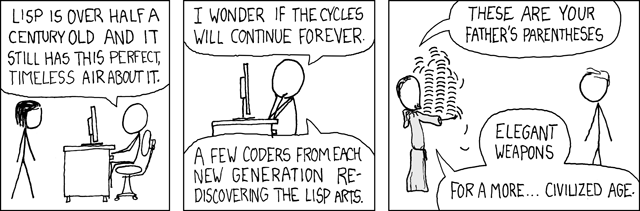
\includegraphics[scale=0.6]{paran.png}
\vspace{1cm}

\newpage

\section{Language description}

\subsection{Data types}
Lithp contains the following data types

\begin{itemize}
    \item Integer
    \item Boolean
    \item String
    \item Atom
    \item List
    \item Nil
    \item Function
\end{itemize}


\subsection{Type System}
Lithp uses a dynamic typing system, meaning that the interpreter determines the type at run time, more specifically at the parsing phase.
Also there are no declaration of the types of variables or functions for that matter making Lithp very vulnerable to type errors.

\subsection{features}
Here is a comprehensive list of all of Lithps functionality:

\begin{itemize}
    \item head: Given a list l returns the head of l.
    \item tail: Given a list l returns the tail of l.
    \item if statements.
    \item functional declaration and application (with recursion!).
\end{itemize}

\section{Implementation}
\subsection{Implementation Language}
I'm by no means fluent or even good at Haskell. I just enjoy functional programming which is one reason I chose to do this in Haskell.
When I got introduced to Haskell programming I really enjoyed it as it taught me a new way of programming and a new way to think.
I've been fond over Haskell ever since then and chose to write Lithp in Haskell due to that fascination and fondness.
I also wanted to pick up concepts in Haskell which I don't understand such as Monads. I had two main issues with this idea though.
First off I didn't really need Monads besides Parsing and IO. The other issue is that although I did get to watch some lectures
and read some notes on Monads, I still didn't really have that much time which could be dedicated to monads.

\subsection{Parsing}
The parsing part of Lithp is "inspired" by "Write yourself a scheme in 48 hours tutorial". By inspired I obviously mean shamelessly
ripped off. Although I've gone through the entire thing slowly to understand the monads at work.

\url{https://en.wikibooks.org/wiki/Write_Yourself_a_Scheme_in_48_Hours/Parsing}

Note: Lithp and the end product of that tutorial are implemented vastly different. The tutorial actually provides a decent programming language.
The only parts that are similar are the parsing.
\end{document}
